\documentclass{article}
\usepackage[margin=1in]{geometry}
\usepackage{enumitem}
\usepackage{setspace}
\usepackage{amsmath}
\usepackage{amssymb}
\usepackage{physics}
\usepackage{graphicx}

\title{Math 180 Homework 2}
\date{10/16/2020}
\author{Jiaping Zeng}

\begin{document}
\setstretch{1.35}
\maketitle

\begin{itemize}
    \item [4.4.7]
          \begin{itemize}
              \item [(a)] \textbf{Answer:} All of the graphs have a Hamiltonian cycle as shown below.
                    \begin{center}
                        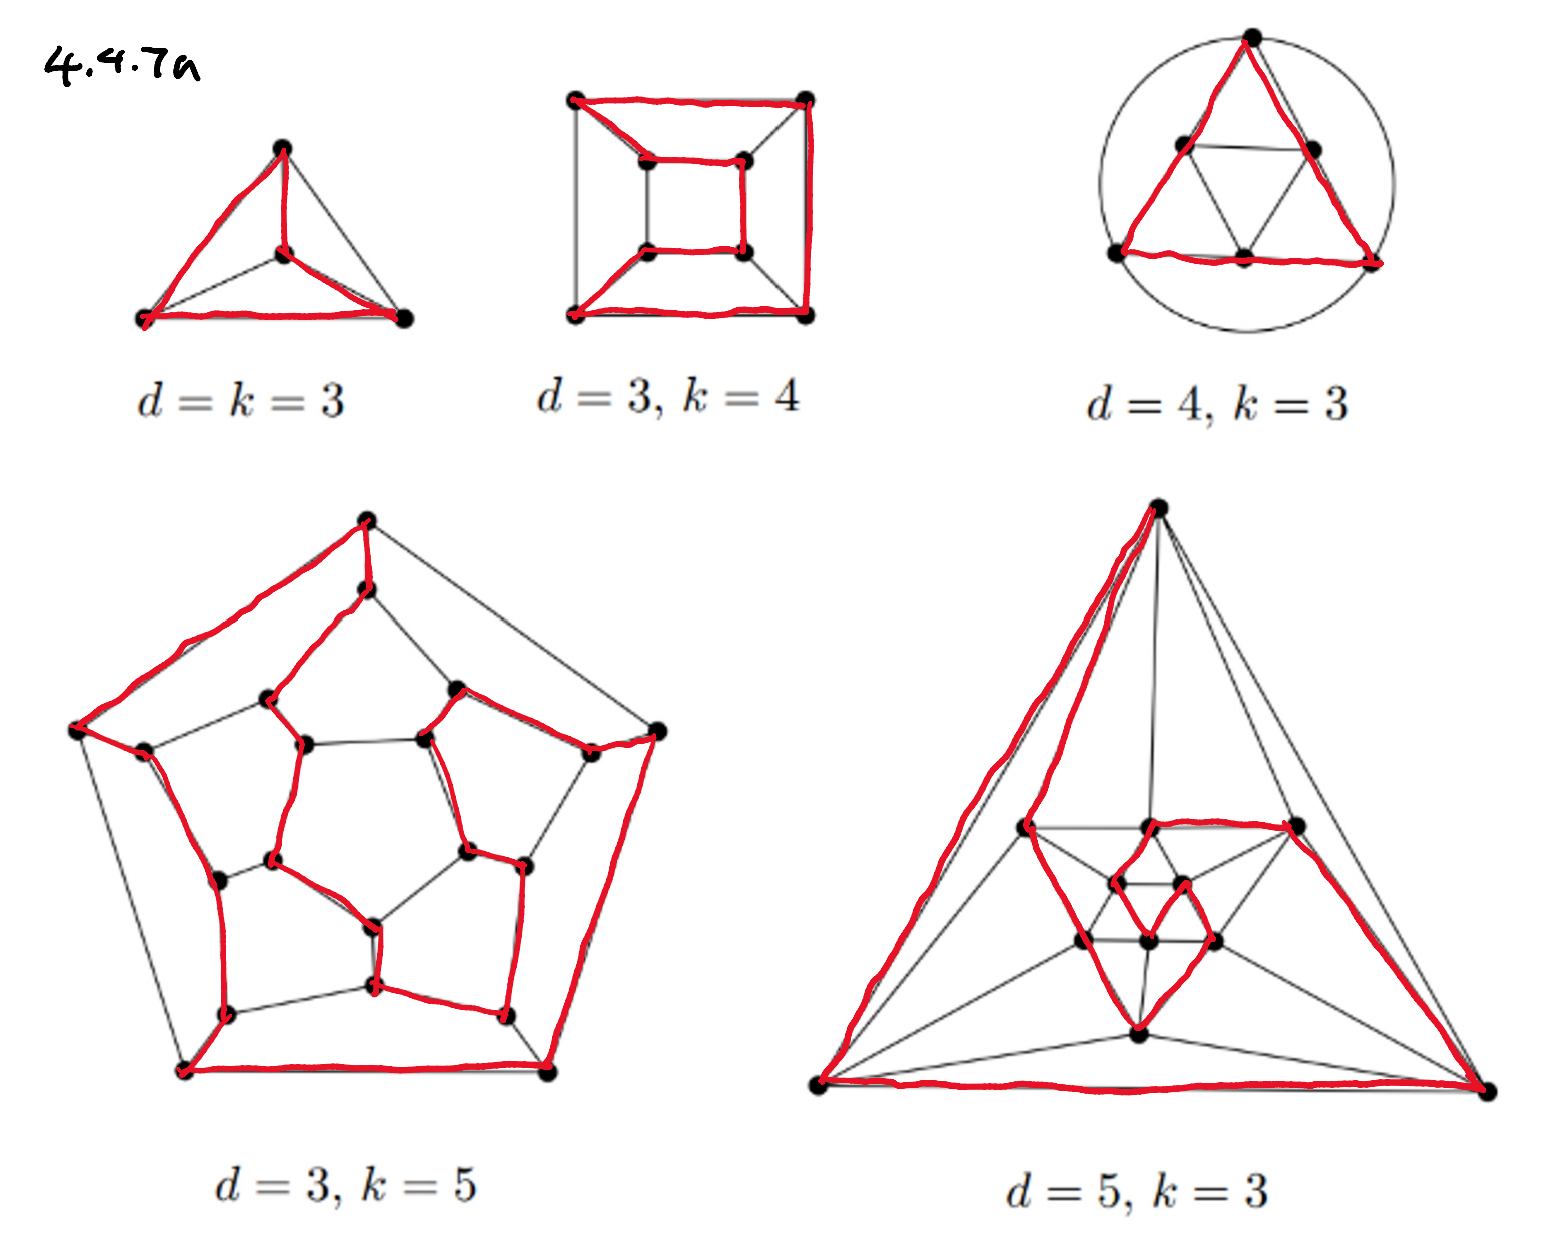
\includegraphics[width=4in]{4-4-7a.png}
                    \end{center}
              \item [(b)] \textbf{Answer:} As shown below, both graphs have score $(3,3,2,2,2,2)$. The bottom one has a Hamiltonian cycle whereas the top one does not.
                    \begin{center}
                        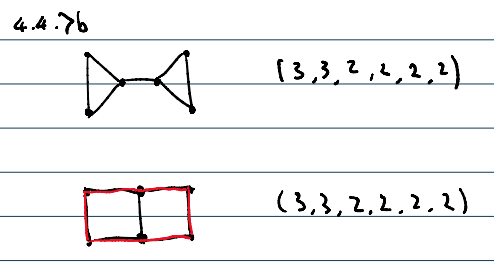
\includegraphics[width=3in]{4-4-7b.png}
                    \end{center}
          \end{itemize}
    \item [4.4.8]
          \begin{itemize}
              \item [(a)] $G$ is connected if and only if $L(G)$ is connected.\\
                    \textbf{Answer: True}, Proof:
                    \begin{itemize}
                        \item [$\Rightarrow$:] Since $G$ is connected, we can select arbitrary vertices $u,v$ and there must exist a path between them. Let $\{w_1,\ldots,w_n\}$ be the vertices on the path, then $(u,w_1),(w_2,w_3),\ldots,(w_n,v)$ are edges in $G$. By definition of line graph, $(u,w_1),(w_2,w_3),\ldots,(w_n,v)$ are vertices in $L(G)$ and $\{w_1,\ldots,w_n\}$ are edges. Then arbitrary vertices $(u,w_1)$ and $(w_n,v)$ in $L(G)$ are connected by edges $\{w_1,\ldots,w_n\}$, i.e. $L(G)$ is connected.
                        \item [$\Leftarrow$:] Since $L(G)$ is connected, we can select two arbitrary vertices $(u,w_1),(w_n,v)$ and there must exist a path between them. Let vertices between them be $(w_1,w_2),\ldots,(w_{n-1},w_n)$ and the edges $\{w_1,\ldots,w_n\}$. Then in graph $G$, vertices $\{w_1,\ldots,w_n\}$ are connected by edges $(w_1,w_2),\ldots,(w_{n-1},w_n)$, i.e. there exist a path between arbitrary vertices $w_1$ and $w_n$. Therefore $G$ is connected by definition.
                    \end{itemize}
              \item [(b)] $G$ is Eulerian if and only if $L(G)$ has a Hamiltonian cycle.\\
                    \textbf{Answer: False}; by counter example: $K_4$ and $L(K_4)$. $K_4$ is not Eulerian as its vertices are odd degrees; whereas $L(K_4)$ has a Hamiltonian cycle as shown in the diagram below.
                    \begin{center}
                        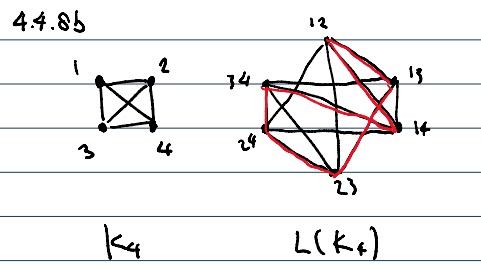
\includegraphics[width=3in]{4-4-8b.png}
                    \end{center}
          \end{itemize}
    \item [4.5.8] \textbf{Answer:} By induction.\\
          Base case: Consider a tournament with exactly two vertices $u,v$, then either $(u,v)$ is present in the graph or $(v,u)$ is. If $(u,v)$ is present, $u\rightarrow v$ is a Hamiltonian path; if $(v,u)$ is present, $v\rightarrow u$ is a Hamiltonian path.\\
          Inductive step: Assume that each tournament with $n>2$ vertices has a Hamiltonian path. Take arbitrary vertex $v$, we can separate the other vertices in the tournament into two tournaments, $T_1$ and $T_2$, such that $T_1$ contains vertices with a directed to $v$ and $T_2$ contains vertices with a directed edge from $v$. Since $T_1$ and $T_2$ are tournaments with sizes smaller than $n$, they must both contain Hamiltonian cycles. Then we can simply take a path in $T_1$ and connect it to a path in $T_2$ by $v$, constructing a Hamiltonian path. Therefore each tournament has a Hamiltonian path by mathematical induction.
    \item [4.6.5] \textbf{Answer:} $Q_k$ is $k$-connected. Proof by induction:\\
          Base case: Since $Q_2$ is a square, we can remove any one of its vertices and obtain a connected path of length 3. Therefore $Q_2$ is $2$-connected.\\
          Inductive step: Assume $Q_n$ is $n$-connected, we want to show that $Q_{n+1}$ is $(n+1)$-connected. Since $Q_{n+1}$ can be constructed by "moving" $Q_k$ into an additional dimension, it could also be thought of as two connected $Q_n$. Then, we would need to remove $n$ vertices from one of the $Q_n$ by the inductive hypothesis, then remove an extra vertex to separate the two $Q_n$. Therefore $Q_{n+1}$ is $(n+1)$ connected and $Q_k$ is $k$-connected by mathematical induction.
    \item [P4] Prove that $K_{p,q}$ does not have a Hamiltonian cycle if $p\neq q$.\\
          \textbf{Answer:} We can define the vertex set of $K_{p,q}$ by $V(K_{p,q})=X\cup Y$, where $X=\{x_1,\ldots,x_p\}$ and $Y=\{y_1,\ldots,y_q\}$. Then the edge set can be defined as $E=\{\{x_i,y_j\}\mid 1\leq i\leq p, 1\leq j\leq q\}$. Note that $p\neq q$; we can assume $p<q$ upon renaming the sets. We can attempt to construct a Hamiltonian cycle as follows: start at  vertex $x_1$ (this choice is arbitrary since we can renumber the vertices). Then the next vertex on the cycle must be in the set $Y$ since $x_a$ is only connected to vertices in $Y$; choose $y_1$ (arbitrary upon renumbering) here. Similarly, the next vertex must be in the set $X$ and must also not be $x_1$; choose $x_2$. Repeat this process until we reach $x_p$ and then $y_p$. From $y_p$, the next vertex in the cycle must be in the set $X$, yet every vertex in $X$ is already in the path so far. In other words, the set of vertices $\{y_{p+1},\ldots,y_q\}$ will never be reached, therefore it is not possible to construct a Hamiltonian cycle from $K_{p,q}$ with $p\neq q$.
    \item [P6] Suppose a graph $G$ on $n\geq 2$ vertices has at least $\frac{(n-1)(n-2)}{2}+1$ edges. Prove that $G$ is connected.\\
          \textbf{Answer:} Suppose we can construct a disconnected graph with $n\geq 2$ vertices and $\frac{(n-1)(n-2)}{2}+1$ edges. By problem 4.2.2 from the previous homework, the maximum possible number of edges with $n$ vertices and 2 components is constructed with $K_{n-1}$ and a single vertex. Take $n-1$ vertices; we can try to "use up" as many edges as possible by constructing a complete graph $K_{n-1}$, which contains $\frac{(n-1)(n-2)}{2}$ edges. However, we still have one edge remaining, meaning that the last edge must be connected to $u$. Then this constructed graph is connected which contradicts the initial assumption of $G$ being disconnected. Therefore $G$ is connected.
    \item [P7] Consider the $k$-dimensional hypercube graph $Q_k$.\begin{itemize}
              \item [1.] What is $\abs{V(Q_k)}$?\\
                    \textbf{Answer:} $2^k$ since there are $2^k$ possible combinations of $0$s and $1$s in a $k$-length sequence.
              \item [2.] What is $\abs{E(Q_k)}$?\\
                    \textbf{Answer:} $k2^{k-1}$. Each vertex has $k$ edges, so we can find the number of edges by halving the sum of the degrees, i.e. $\frac{k2^k}{2}=k2^{k-1}$.
              \item [3.] What is the \textit{diameter} (maximal distance between any two vertices) of $Q_k$?\\
                    \textbf{Answer:} $k$. Since two sequences can only differ by one coordinate at a time, the distance between the $k$-length sequence of all $0$s and the $k$-length sequence of all $1$s is $k$.
              \item [4.] Prove that $Q_k$ is bipartite.\\
                    \textbf{Answer:} By construction, the vertex set is all sequences of $0$s and $1$s of length $k$, where two sequences are adjacent if and only if they differ in exactly one coordinate. As a result, we can simply separate the vertices into two sets, one with an even number of $1$s and the other with an odd number of $1$s. Since two vertices are only adjacent if they different in exactly one coordinate, any element in the first set is only adjacent to elements in the second set and vise versa. Therefore $Q_k$ is bipartite.
          \end{itemize}
\end{itemize}
\end{document}